\section{Bayesian Analysis}

\subsection{Initial Setup - Choosing a Prior and Modeling Data}
For our analysis purpose, we divided our data into 2 parts of 6 months.
From the first 6 months of data, we built our prior knowledge by calculating its mean and variance.
We model the data assuming it follows a normal distribution with known mean.
Hence, data $X | \mu \sim N(\mu, \sigma^2)$, where $\sigma^2$ is known.
$$ f(x | \mu) = \frac{1}{\sigma \sqrt{2\pi}} \exp\left(-\frac{(x - \mu)^2}{2\sigma^2}\right) $$
We take the variance of our model to be the sample variance of the known data, where $\mu_x$ is the sample mean of the known data.
        $$ S^2 = \sum_{i = 1}^{n} \frac{(x_i - \mu_x)^2}{n - 1} $$
We supposed $\mu \sim N(u, v)$ is the prior distribution of $\mu$.
The likelihood function, given the sample $\bar{x} = (x_1, x_2, \dots, x_n)$, can be calculated as: $$ L(\mu | \bar{x}) = \prod_{i = 1}^{n} f(x_i | \mu)$$
The posterior distribution will be: $$ \propto \exp\left(-\frac{1}{2v'} (\mu - u')^2\right)$$
where $u' = \left(u \sigma^2 + v \sum_{i = 1}^{n} x_i\right) / (n v + \sigma^2)$ and $v' = v \sigma^2/(n v + \sigma^2)$.
By the kernel of the posterior distribution, it is evident that $\mu | \bar{x} \sim N(u', v')$.



\subsection{Updating the Prior Month-by-Month}

    The posterior for current month reflects our updated belief about the product's revenue after observing current month sales.
    For each subsequent month, we treat the posterior from the previous month as the new prior.
    This recursive process allows us to carry forward accumulated information, refining our estimate of the product's revenue month after month as we get more and more data.
Here, we visualize the evolution of the posterior distributions over each month.
These distributions become more concentrated, indicating increased confidence as more data is incorporated over time.
\begin{figure}[!ht]
  \centering
  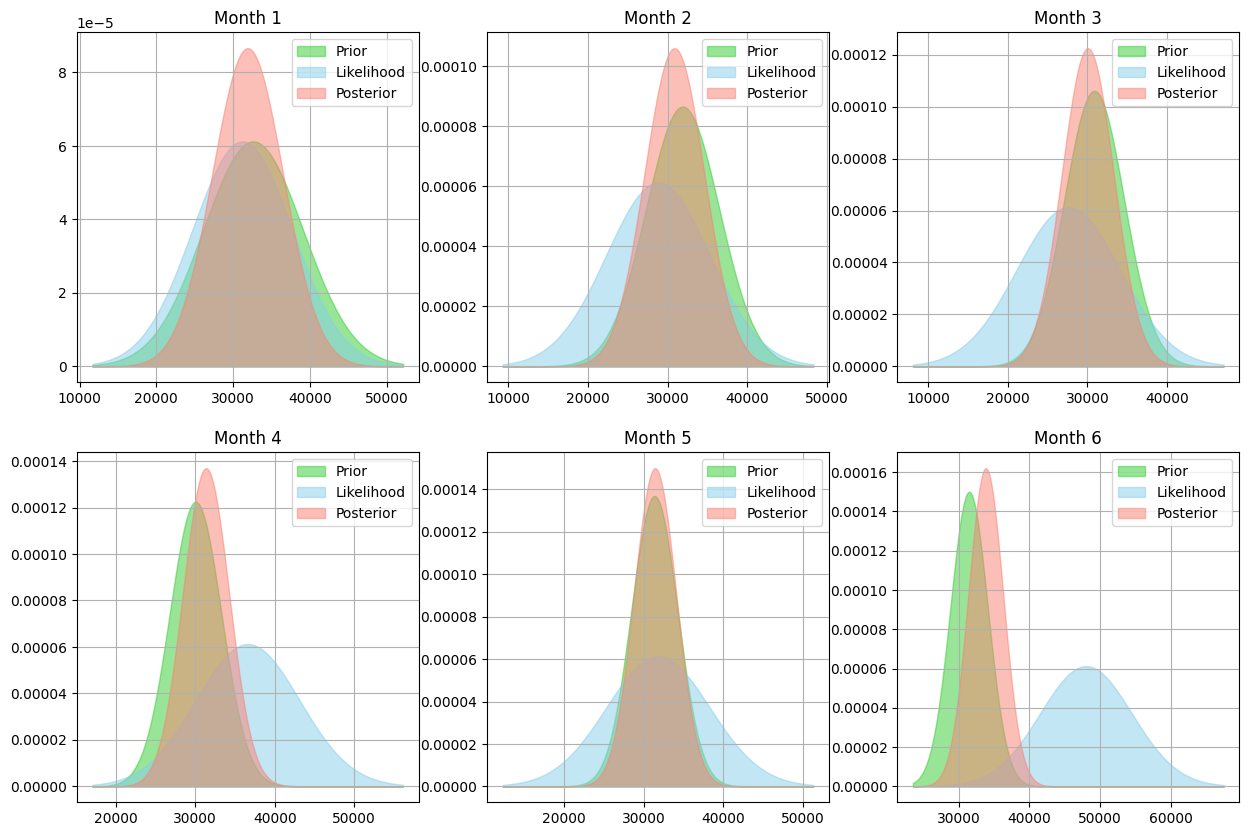
\includegraphics[width=.6\textwidth]{images/months.png}
  \caption{Prior, Likelihood, and Posterior for each month}
\end{figure}


\subsection{Reporting Posterior Metrics}

By the end of 1 year, we report key metrics from the final posterior distribution. \\
95\% Confidence Interval: The range where the revenue estimate is most likely to lie. \\
Posterior Mean: The expected revenue estimate based on all months of data. \\
Variance: Reflects our confidence in this estimate; lower variance implies greater certainty.

\begin{figure}[!ht]
  \centering
  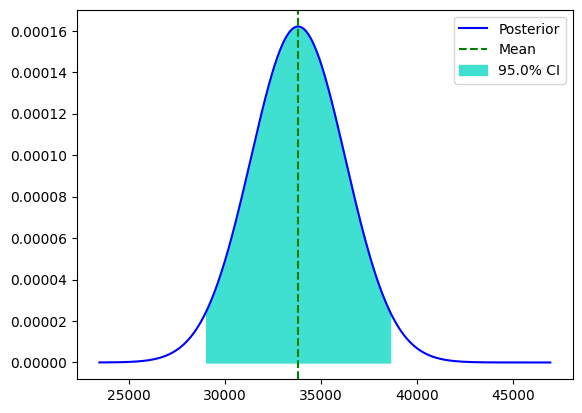
\includegraphics[width=.6\textwidth]{images/ci.png}
  \caption{95\% Confidence Interval}
\end{figure}

\subsection{Posterior Mean and Variance Analysis}

The posterior mean over time shows how our estimate of revenue has evolved.
A decreasing variance suggests that our confidence is increasing, as we have more data to base our estimates on.
These metrics help us assess how consistent the product's revenue has been over time.

\begin{figure}[!ht]
  \centering
  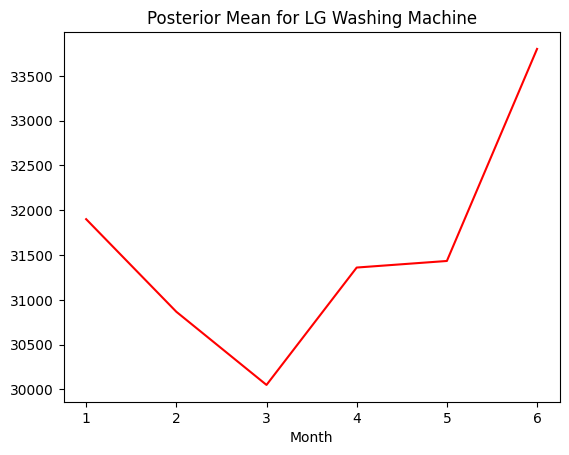
\includegraphics[width=.5\textwidth]{images/mean.png}
  \caption{Posterior mean for each month}
\end{figure}

\begin{figure}[!ht]
  \centering
  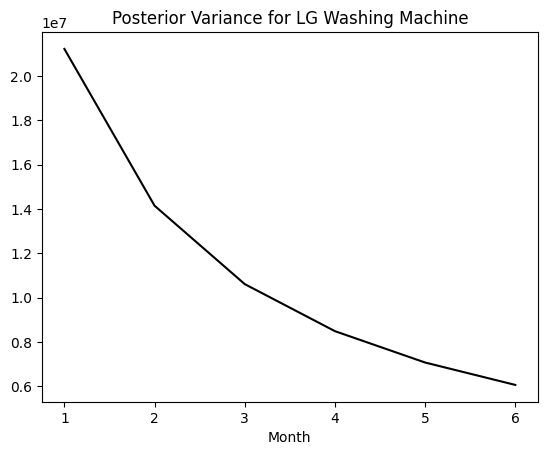
\includegraphics[width=.5\textwidth]{images/var.png}
  \caption{Posterior variance for each month}
\end{figure}
